\documentclass[12pt, a4paper]{report}
\usepackage[top=1cm, left=1cm, right=1cm]{geometry}

\usepackage[utf8]{inputenc}
\usepackage[russian]{babel}

\usepackage{array}
\newcolumntype{M}[1]{>{\centering\arraybackslash}m{#1}}

\usepackage{hyperref}
\hypersetup{
	colorlinks,
	citecolor=black,
	filecolor=black,
	linkcolor=black,
	urlcolor=black
}

\usepackage{sectsty}
\allsectionsfont{\centering}

\usepackage{indentfirst}
\setlength\parindent{24pt}

\usepackage{makecell}

\usepackage{amsmath}

\usepackage{tikz}
\usetikzlibrary{shapes.geometric, arrows}

\usepackage{listings}
\usepackage{xcolor}
\definecolor{codegreen}{rgb}{0,0.6,0}
\definecolor{codegray}{rgb}{0.5,0.5,0.5}
\definecolor{codepurple}{rgb}{0.58,0,0.82}
\definecolor{backcolour}{rgb}{0.95,0.95,0.92}
\lstdefinestyle{mystyle}{
    backgroundcolor=\color{backcolour},
    commentstyle=\color{codegreen},
    keywordstyle=\color{magenta},
    numberstyle=\normalsize\color{codegray},
    stringstyle=\color{codepurple},
    basicstyle=\ttfamily\footnotesize,
    breakatwhitespace=false,
    breaklines=true,
    captionpos=b,
    keepspaces=true,
    numbers=left,
    numbersep=5pt,
    showspaces=false,
    showstringspaces=false,
    showtabs=false,
    tabsize=2
}

\usepackage{graphicx}
\graphicspath{ {plots/pictures/} }

\begin{document}
	\begin{titlepage}
		\begin{center}
			\large \textbf{Министерство науки и высшего образования Российской Федерации} \\
			\large \textbf{Федеральное государственное бюджетное образовательное учреждение высшего образования} \\
			\large \textbf{«Российский химико-технологический университет имени Д.И. Менделеева»} \\

			\vspace*{4cm}
			\LARGE \textbf{ОТЧЕТ ПО ЛАБОРАТОРНОЙ РАБОТЕ №1}

			\vspace*{1cm}
			\LARGE \textbf{Вариант 22}

			\vspace*{4cm}
			\begin{flushright}
				\Large
				\begin{tabular}{>{\raggedleft\arraybackslash}p{9cm} p{10cm}}
					Выполнил студент группы КС-36: & Золотухин А.А. \\
					Ссылка на репозиторий: & https://github.com/ \\
					& CorgiPuppy/ \\
					& num-methods-eq-math-phys-chem-labs \\
					Принял: & Лебедев Данила Александрович \\
					Дата сдачи: & 02.04.2025 \\
				\end{tabular}
			\end{flushright}

			\vspace*{4cm}
			\Large \textbf{Москва \\ 2025}
		\end{center}
	\end{titlepage}

	\tableofcontents
	\thispagestyle{empty}
	\newpage

	\pagenumbering{arabic}

	\section*{Описание задачи}
	\addcontentsline{toc}{section}{Описание задачи}
	\large
	\begin{center}
		\begin{tabular}{||c|c|c|c||}
			\hline
			Вариант & Уравнение & Интервалы переменных & Начальные и граничные условия \\
			\hline
			22 & $ \frac{\partial u}{\partial t}=\frac{\partial^2 u}{\partial x^2}$ & \makecell{$ x \in [0, 1] $ \\ $ t \in [0, 1] $} & \makecell{$ u(t = 0, x) = e^x $ \\ $ u(t, x = 0) = e^t $ \\ $ u(t, x = 1) = e^{t+1} $} \\

			\hline
		\end{tabular}
	\end{center}
	\par
	Для заданного уравнения:
	\begin{enumerate}
		\item записать явную разностную схему;
		\item определить порядок аппроксимации разностной схемы;
		\item получить условие устойчивости разностной схемы на шаг (с помощью метода гармоник);
		\item вывести рекуррентное соотношение;
		\item составить алгоритм (блок-схему) расчёта;
		\item построить программу на любом удобном языке программирования;
		\item провести численный расчёт с использованием различных значений $ \Delta t (0.1, 0.01, 0.001)$, $ h = 0.1 $;
		\item составить отчёт о проделанной работе.
	\end{enumerate}
	\newpage

	\section*{Выполнение задачи}
	\addcontentsline{toc}{section}{Выполнение задачи}

	\subsection*{Задание 1}
	\addcontentsline{toc}{subsection}{Задание 1}
	\large
	Записать явную разностную схему:
	\begin{equation}\label{eq:explicit}
		\frac{u_{j}^{n+1}-u_{j}^{n}}{\Delta t}=\frac{u_{j+1}^{n}-2u_{j}^{n}+u_{j-1}^{n}}{h^{2}}.
	\end{equation}	
	\par
	В записанной разностной схеме \eqref{eq:explicit} аппроксимация второй производной функции \textit{u(t, x)} по координате рассматривается на \textit{n}-м шаге по времени, т.е. относительно точки $t^{n}$, для которой рассматривается аппроксимация всего уравнения. Такая разностная схема называется \textbf{явной}.

	\subsection*{Задание 2}
	\addcontentsline{toc}{subsection}{Задание 2}
	\large
	Определить порядок аппроксимации разностной схемы \eqref{eq:explicit}: \par
	Для этого запишу разложение значений $u_{j}^{n+1}$, $u_{j+1}^{n}$, $u_{j-1}^{n}$ в ряд Тейлора относительно точки ($t^{n}$, $x_{j}$) на разностной сетке:
	\begin{equation}\label{eq:value1}
		u_{j}^{n+1} = u_{j}^{n} + \left.\frac{\partial u}{\partial t}\right|_{j}^{n}\Delta t + \left.\frac{1}{2!}\frac{\partial^{2} u}{\partial t^{2}}\right|_{j}^{n}(\Delta t)^{2} + \left.\frac{1}{3!}\frac{\partial^{3} u}{\partial t^{3}}\right|_{j}^{n}(\Delta t)^{3} + \dots,
	\end{equation}
	\begin{equation}\label{eq:value2}
		u_{j+1}^{n} = u_{j}^{n} + \left.\frac{\partial u}{\partial x}\right|_{j}^{n}h + \left.\frac{1}{2!}\frac{\partial^{2} u}{\partial x^{2}}\right|_{j}^{n}h^{2} + \left.\frac{1}{3!}\frac{\partial^{3} u}{\partial x^{3}}\right|_{j}^{n}h^{3} + \left.\frac{1}{4!}\frac{\partial^{4} u}{\partial x^{4}}\right|_{j}^{n}h^{4} + \dots,
	\end{equation}
	\begin{equation}\label{eq:value3}
		u_{j-1}^{n} = u_{j}^{n} - \left.\frac{\partial u}{\partial x}\right|_{j}^{n}h + \left.\frac{1}{2!}\frac{\partial^{2} u}{\partial x^{2}}\right|_{j}^{n}h^{2} - \left.\frac{1}{3!}\frac{\partial^{3} u}{\partial x^{3}}\right|_{j}^{n}h^{3} + \left.\frac{1}{4!}\frac{\partial^{4} u}{\partial x^{4}}\right|_{j}^{n}h^{4} - \dots.
	\end{equation}
	\par
	Подставляя зависимости \eqref{eq:value1}-\eqref{eq:value3} в разностную схему \eqref{eq:explicit}, получаем:
	\begin{equation*}
		\left.\frac{\partial u}{\partial t}\right|_{j}^{n} + \left.\frac{1}{2}\frac{\partial^{2} u}{\partial t^{2}}\right|_{j}^{n}\Delta t + \left.\frac{1}{6}\frac{\partial^{3} u}{\partial t^{3}}\right|_{j}^{n}(\Delta t)^{2} = \left.\frac{\partial^{2} u}{\partial x^{2}}\right|_{j}^{n} + \left.\frac{1}{12}\frac{\partial^{4} u}{\partial x^{4}}\right|_{j}^{n}h^{2}.
	\end{equation*}
	\begin{equation*}
		\Rightarrow \left.\frac{\partial u}{\partial t}\right|_{j}^{n} + O(\Delta t) = \left.\frac{\partial^{2} u}{\partial x^{2}}\right|_{j}^{n} + O(h^{2}).
	\end{equation*}
	\par
	Таким образом, явная разностная схема \eqref{eq:explicit} аппроксимирует исходное дифференциальное уравнение с первым порядком по времени и со вторым порядком по координате, что записывается в следующем виде:
	\begin{equation*}
		O(\Delta t) + O(h^{2}) \text{ или } O(\Delta t, h^{2}).
	\end{equation*}

	\subsection*{Задание 3}
	\addcontentsline{toc}{subsection}{Задание 3}
	\large
	Получить условие устойчивости разностной схемы на шаг (с помощью метода гармоник): \par
	Представлю решение разностной схемы в виде гармоники:
	\begin{equation}\label{eq:harmonic}
		u_{j}^{n} = \lambda^{n}e^{i \alpha j}.
	\end{equation}
	\par
	Подставляя \eqref{eq:harmonic} в разностную схему \eqref{eq:explicit}, получаю:
	\begin{equation*}
		\frac{\lambda^{n+1}e^{i \alpha j} - \lambda^{n}e^{i \alpha j}}{\Delta t} = \frac{\lambda^{n}e^{i \alpha (j+1)} - 2\lambda^{n}e^{i \alpha j} + \lambda^{n}e^{i \alpha (j-1)}}{h^{2}}.
	\end{equation*}
	\par
	Упрощаю полученное выражение, деля левую и правую его части на $\lambda^{n}e^{i \alpha j}$:
	\begin{equation*}
		\frac{\lambda - 1}{\Delta t} = \frac{e^{i \alpha} - 2 + e^{-i \alpha}}{h^{2}}.
	\end{equation*}
	\par
	Преобразую комплексные числа из экспоненциальной формы в тригонометрическую:
	\begin{equation*}
		e^{\pm i \alpha} = \cos{\alpha} \pm i\sin{\alpha} \Rightarrow \frac{\lambda - 1}{\Delta t} = \frac{2\cos{\alpha} - 2}{h^{2}}.
	\end{equation*}
	\par
	Используя тригонометрические тождества
	\begin{equation*}
		\cos{\alpha} = \cos^{2}{\frac{\alpha}{2}} - \sin^{2}{\frac{\alpha}{2}} = 1 - 2\sin^{2}{\frac{\alpha}{2}},
	\end{equation*}
	получаю формулу, из которой затем выражаю $\lambda$:
	\begin{equation*}
		\frac{\lambda - 1}{\Delta t} = \frac{-4\sin^{2}{\frac{\alpha}{2}}}{h^{2}} \Rightarrow \lambda = 1 - \frac{4 \Delta t}{h^{2}}\sin^{2}{\frac{\alpha}{2}}.
	\end{equation*}
	\par
	С учётом необходимого условия устойчивости разностных схем $\lvert \lambda \rvert \leq 1$ имею:
	\begin{equation*}
		-1 \leq 1 - \frac{4 \Delta t}{h^{2}}\sin^{2}{\frac{\alpha}{2}} \leq 1.
	\end{equation*}
	\par
	В полученном двойном неравенстве правое условие выполняется автоматически. Поэтому рассмотрю более подробно левое условие:
	\begin{equation*}
		1 - \frac{4 \Delta t}{h^{2}}\sin^{2}{\frac{\alpha}{2}} \geq -1 \Rightarrow \frac{\Delta t}{h^{2}}\sin^{2}{\frac{\alpha}{2}} \leq \frac{1}{2}.
	\end{equation*}
	\par
	Задавая для $\sin^{2}{\frac{\alpha}{2}}$ максимально возможное значение, равное 1, перехожу к более строгому условию, справедливому для любого $\alpha$:
	\begin{equation}\label{eq:stability}
		\frac{\Delta t}{h^{2}}\sin^{2}{\frac{\alpha}{2}} \leq \frac{1}{2} \Rightarrow \frac{\Delta t}{h^{2}} \leq \frac{1}{2}.
	\end{equation}
	\par
	Выражение \eqref{eq:stability} является условием устойчивости явной разностной схемы, аппроксимирующей одномерное дифференциальное уравнение параболического типа. Такие разностные схемы, устойчивость которых зависит от какого-либо условия, ограничивающего выбор интервала деления на разностной сетке, называют \textbf{условно устойчивыми}. \par
	При $h = 10^{-1}$:
	\begin{equation*}
		\Delta t \leq \frac{(10^{-1})^{2}}{2} \Rightarrow \Delta t \leq 5 \cdot 10^{-3}.
	\end{equation*}

	\subsection*{Задание 4}
	\addcontentsline{toc}{subsection}{Задание 4}
	\large
	Вывести рекуррентное соотношение: \par
	Выражаю из разностной схемы \eqref{eq:explicit} величину $u_{j}^{n+1}$:
	\begin{equation}\label{eq:recurrence}
		u_{j}^{n+1} = u_{j}^{n} + \frac{\Delta t}{h^{2}}(u_{j+1}^{n} - 2u_{j}^{n} + u_{j-1}^{n}).
	\end{equation}
	\par
	Соотношение типа \eqref{eq:recurrence}, позволяющее рассчитывать значения искомой функции в узлах разностной сетки через известные значения в других узлах разностной сетки, называют \textbf{рекуррентным соотношением}.

	\subsection*{Задание 5}
	\addcontentsline{toc}{subsection}{Задание 5}
	\large
	Составить алгоритм (блок-схему) расчёта: \par
	\tikzstyle{start} = [circle, draw=black!60, fill=white!5, very thick, minimum size=10mm]
	\tikzstyle{stop} = [circle, color=black!60, fill=black!60, very thick, minimum size=10mm]
	\tikzstyle{process} = [rectangle, minimum width=3cm, minimum height=1cm, text centered, draw=black]
	\tikzstyle{decision} = [diamond, minimum width=3cm, minimum height=1cm, text centered, draw=black]
	\tikzstyle{arrow} = [thick,->,>=stealth]
	\begin{center}
		\begin{tikzpicture}[node distance=2cm]
			\node (start) [start] {};
			\node (in1) [process, below of=start] {\makecell{Задание начальных условий: \\ цикл по $j=1..N_{x}$ \\ $u_{j}^{0} = e^{(j - 1)h}$}};
			\node (in2) [process, below of=in1] {$n = 0$};
			\node (dec) [decision, below of=in2, yshift=-1cm] {$n = N_{t}$};
			\node (stop) [stop, right of=dec, xshift=2cm] {};
			\node (pr1) [process, below of=dec, yshift=-1cm] {\makecell{цикл по $j=2..N_{x}-1$ \\ $u_{j}^{n+1} = u_{j}^{n} + \frac{\Delta t}{h^{2}}(u_{j+1}^{n} - 2u_{j}^{n} + u_{j-1}^{n})$ }};
			\node (pr2) [process, below of=pr1, yshift=-1cm] {\makecell{Определение $u_{1}^{n+1}$ и $u_{N_{x}}^{n+1}$ из граничных условий \\ $u_{1}^{n+1} = e^{(n + 1)\Delta t}$ \\ $u_{N_{x}}^{n+1} = e^{(n + 1)\Delta t + 1}$}};
			\node (pr3) [process, below of=pr2, yshift=-1cm] {$n = n + 1$};
			\draw [arrow] (start) -- (in1);
			\draw [arrow] (in1) -- (in2);
			\draw [arrow] (in2) -- (dec);
			\draw [arrow] (dec) -- node[anchor=south] {да} (stop);
			\draw [arrow] (dec) -- node[anchor=west] {нет} (pr1);
			\draw [arrow] (pr1) -- (pr2);
			\draw [arrow] (pr2) -- (pr3);
			\draw [arrow] (pr3.west) -- ++(left:5cm) -| +(up:9cm) -- (dec.west);
		\end{tikzpicture}
	\end{center}

	\subsection*{Задание 8}
	\addcontentsline{toc}{subsection}{Задание 8}
	\large
	Построить программу на любом удобном языке программирования:
	\lstset{style=mystyle}
	\lstinputlisting[language=C++]{src/main.cpp}

	\subsection*{Задание 8}
	\addcontentsline{toc}{subsection}{Задание 8}
	\large
	Составить отчёт о проделанной работе. График фукнции \textit{u(t, x)}
	\begin{center}
		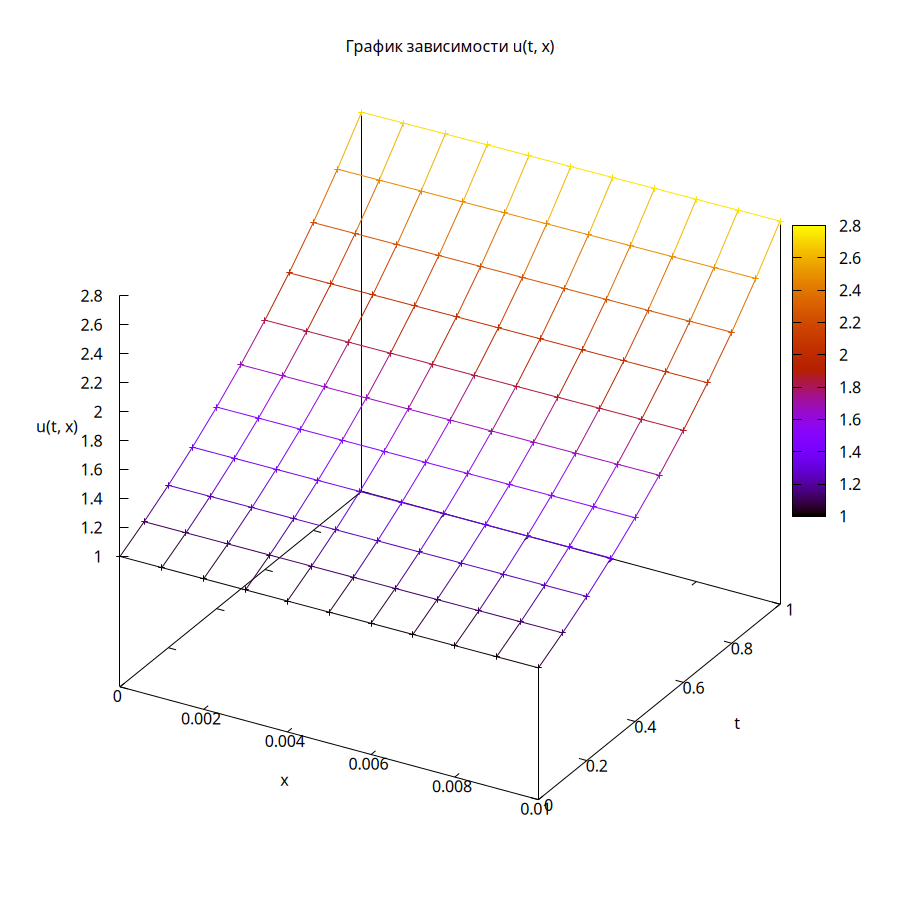
\includegraphics[width=500pt]{u_t_x.png}
	\end{center}
\end{document}
